\section{First Part (Rigid structure from motion by factorization)}
\noindent In this task, factorization for a rigid body must be implemented, as shown in the following slide figure \ref{fig:slideT1}.
\noindent So, we should complete the orthogonal factorization function by means of the file \textbf{rigidfactorization ortho.m}. The completed code runs with a provided test data composed by a synthetic sequence with an Ogre face, and the 3D reconstruction error is reported.\\

\begin{figure}[h]
    \centering
    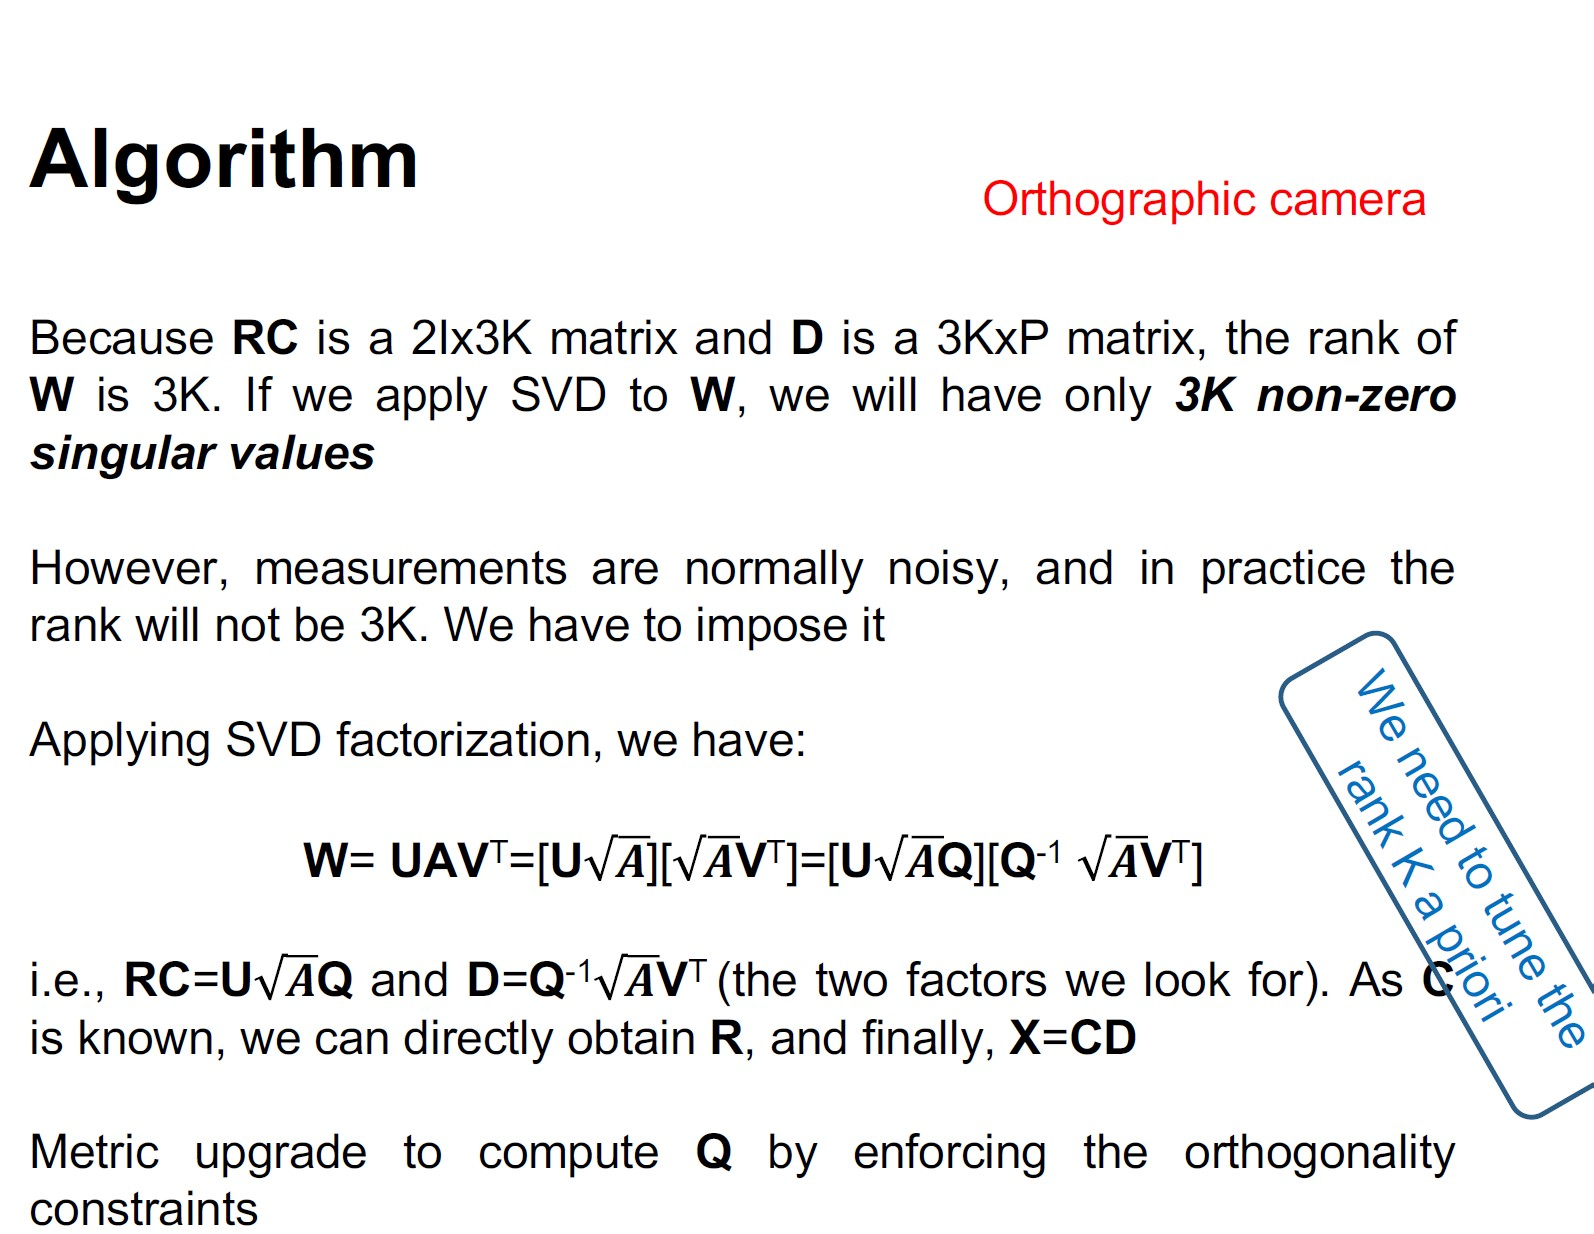
\includegraphics[width=0.75\textwidth]{T1/slide}
    \caption{Factoring slide}
    \label{fig:slideT1}
\end{figure}

\subsection{Code:}
\noindent Now, we introduce the code \ref{lstlisting-codeT1}. We will explain each line number:\\ 
\noindent For the line $1$ and $2$, $Zc$ is defined as the difference between the input matrix and the average of all the points in each frame, and not as the input matrix.
This way, we no longer have to consider translation in the computations.\\ 
\noindent Therefore, the average matrix would be the following, with dimensions $2f\times p$
\begin{equation}\label{eq:mean}
Mean=
\begin{pmatrix}
Mean_{1} & Mean_{1} & \cdots Mean_{1}\\
Mean_{2} & Mean_{2} & \cdots Mean_{2}\\
\vdots & \vdots & \ddots & \vdots\\
Mean_{f} & Mean_{f} & \cdots Mean_{f}
\end{pmatrix}
\end{equation}
\noindent where
\begin{equation}
Media_{k}=
\begin{pmatrix}
\frac{x_{1} + x_{2} + \cdots + x_{p}}{p}\\
\frac{y_{1} + y_{2} + \cdots + y_{p}}{p}
\end{pmatrix}
\end{equation}
\noindent for any $k$ between $1$ and $f$.
\noindent Therefore from \ref{eq:mean} we have:
\begin{equation}
Zc=Input-Mean
\end{equation}

\noindent In the line "$3$, we calculate the factorization called Singular Value Decomposition (SVD).\\
\noindent In the line $4$ and $5$, we approximate $R=U(:,1:3)D(1:3, 1:3)^{1/2}$ and $S=D(1:3, 1:3)^{1/2}V(:, 1:3)'$ (where $R$ represents rotation and $S$ represents shape). Knowing that the rank of $RS$ is 3, therefore the truth mathix $D$ should have a dimension of $3\times 3$, then we do the following:\\
\begin{itemize}
\item $D$: We take the first 3 rows and the first 3 columns.
\item $U$: We take only the first 3 columns.
\item $V$: We take only the first 3 columns.
\end{itemize}
\noindent therefore in that way we can calculate $S$ as $U_{2I\times 3}\sqrt{D}_{3\times 3}$ and R as $\sqrt{D}_{3\times 3}V^{'}_{3\times 3I}$\\

\noindent In the ``while loop" of the line $10$, we try to reduce $\Vert Zc-RU\Vert$  to the threshold, which in the code is called epsilon. The idea to optimize the rotation matrix is use the rotation condition $R_{i}R_{i}'=I$, where $I$ corresponds to the identity matrix. This rotation condition is used to calculate $T$ in the code and thus be able to calculate the new matrices $S$ and $R$.

\begin{lstlisting}[style=Matlab-editor, numbers=left]
T = mean(Zc,2);
Zc = Zc - repmat(T,1,size(Zc,2)); 
[U, D, V] = svd(Zc);
R = U(:, 1:3)*(D(1:3, 1:3) ^ 1/2); 
S = (D(1:3, 1:3) ^ 1/2)*V(:, 1:3)';
% Metric Upgrade Step
F=size(Zc,1);
k=0;
thenorm=epsilon+1;
while thenorm>epsilon && k<n_iter
    Rp=R;
    M=[];
    for f=1:2:F
       Rf=R(f:f+1,:);
       [U2,useless,V2]=svd(Rf,'econ');       
       T=U2*V2';
       M=[M;T(1:2,:)];
   end 
    S=pinv(M)*Zc;
    R=Zc*pinv(S);
    k=k+1;
    thenorm=norm(R-Rp,'fro')/numel(M);
end
\end{lstlisting}\label{lstlisting-codeT1}
\noindent Finally, ones that the optimization finish, we obtain a shape matrix $S$ to compare as the truth matix shape $X$.

\subsection{Examples:}
\noindent Here we will show how to reconstruct the face of an Ogre with the given frames and using the following input parameters:

\begin{itemize}
\item threholder: $10^{-7}$
\item maximum number of iterations: 200
\end{itemize}

\begin{figure}[h]
    \centering
    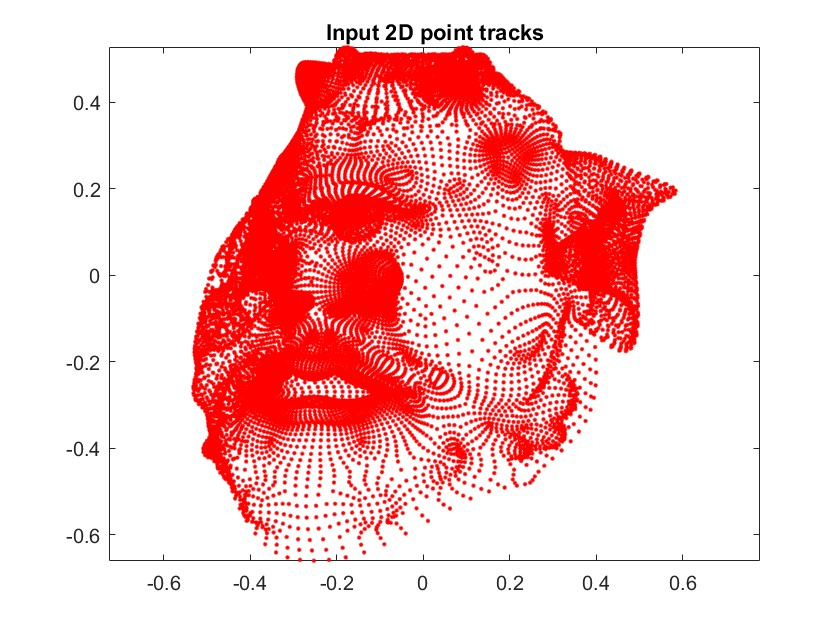
\includegraphics[width=0.6\textwidth]{T1/figure1}
    \caption{The original face of the Ogre.}
    \label{fig:real_ogre}
\end{figure}

\begin{figure}[h]
    \centering
    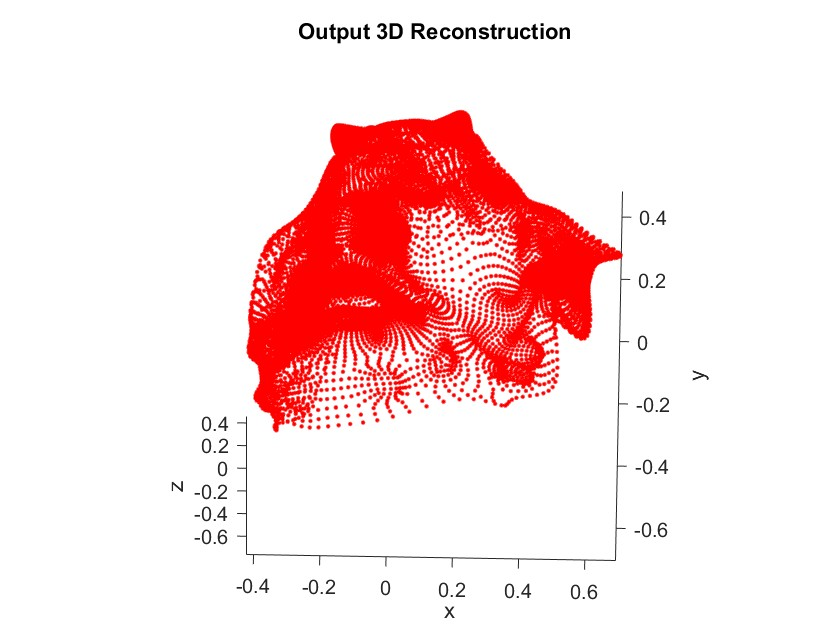
\includegraphics[width=0.75\textwidth]{T1/figure3}
    \caption{The Ogre's face reconstructed by the algorithm.}
    \label{fig:ogre}
\end{figure}

\begin{figure}[h!]
    \centering
    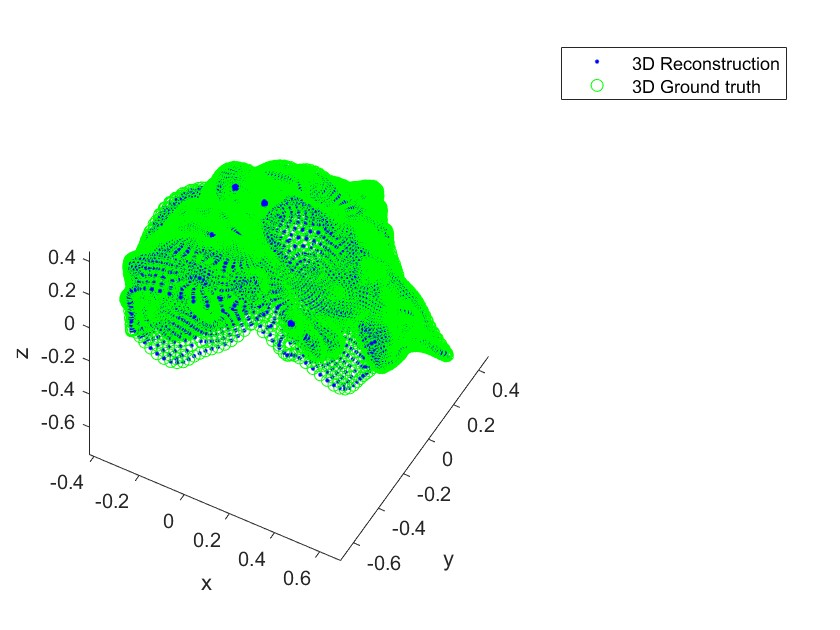
\includegraphics[width=0.75\textwidth]{T1/figure2}
    \caption{Comparison between the 3D representation of the Ogre's original face and its face reconstructed by the algorithm.}
    \label{fig:real_ogre_vs_ogre}
\end{figure}
\noindent As can be seen in Figure \ref{fig:real_ogre_vs_ogre}, the reconstruction of the Ogre's face is quite good. This is demonstrated by the fact that the error between the original Ogre's face and its face reconstructed by the algorithm is 0,0026993\% it means quite low, as depicted Figure \ref{fig:3d_error}.

\begin{figure}[h!]
    \centering
    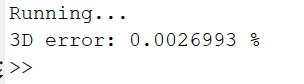
\includegraphics[width=0.4\textwidth]{T1/3derror}
    \caption{Error between the ogre's face and the reconstructed face.}
    \label{fig:3d_error}
\end{figure}
